\documentclass[xcolor=pdftex,dvipsnames,table]{beamer}

%\pdfoptionpdfminorversion=5

\usetheme{default}
\beamertemplatenavigationsymbolsempty

\definecolor{fore}{RGB}{249,242,215}
\definecolor{back}{RGB}{51,51,51}
\definecolor{title}{RGB}{255,0,90}

\setbeamercolor{titlelike}{fg=title}
\setbeamercolor{normal text}{fg=fore,bg=back}

\usepackage[T1]{fontenc}
\usepackage{listings}
%\usepackage{bera}
\usepackage{droid}
\usepackage{eulervm} % for euler math fonts as in concrete math
% \usepackage{luximono} % comment out this line to get droid sans mono

\usepackage[all,tips]{xy}

%%%%%%%%%%%%%%%%%%%%%%%%%%%%%%%%%%%%%%%%%%%%%%%%%%%%%%%%%%%%%%%%%%%%%%
\newcommand{\C}{\ensuremath{\mathcal{C}}}
\renewcommand{\SS}{\ensuremath{\mathcal{S}}}
\newcommand{\id}{\ensuremath{\mathrm{id}}}
\newcommand{\idc}{\ensuremath{\mathrm{id}_\mathcal{C}}}
\newcommand{\typ}{\ensuremath{\mathcal{H}}}
\newcommand{\SET}{\ensuremath{\mathbf{Sets}}}
\newcommand{\Hom}{\ensuremath{\mathrm{Hom}}}
\newcommand{\HSS}[1]{\ensuremath{\Hom( \SS\times\SS ,\SS\times\SS \times #1)}}
\newcommand{\End}{\ensuremath{\mathrm{End}}}
\newcommand{\Endtyp}{\ensuremath{\mathrm{End}(\typ)}}
\newcommand{\Z}{\ensuremath{\mathbb{Z}}}
\newcommand{\bind}{\ensuremath{\mathtt{>>=}}}
\newcommand{\shove}{\ensuremath{\mathtt{>>>}}}
%%%%%%%%%%%%%%%%%%%%%%%%%%%%%%%%%%%%%%%%%%%%%%%%%%%%%%%%%%%%%%%%%%%%%%

\newcommand{\hili}[1]{\emph{\textcolor{title}{#1}}}

\definecolor{keywords}{RGB}{255,0,90}
\definecolor{comments}{RGB}{60,179,113}
\lstset{language=Haskell,
keywordstyle=\color{keywords},
commentstyle=\color{comments}\emph,
basicstyle=\ttfamily}

\setbeamertemplate{itemize item}{$\star$}

\title{Mathematically Structured Computer Programs}
%\subtitle{subtitle}
\author{Sreekar M. Shastry}
\date{28 February 2011}

\begin{document}

\begin{frame}
    \titlepage{}
\end{frame}

\begin{frame}[fragile]
\setbeamercovered{dynamic}
\begin{verbatim}
    int f(int n)
    {
        return n + CurrentSecond()
    }
\end{verbatim}    \pause

\begin{itemize}
    \item The type signature, \verb|int f(int n)|, suggests that
        \verb|f| is a function from the integers to itself, in the
        mathematical sense. \pause
    \item But of course it is not.
\end{itemize}
\end{frame}

\begin{frame}
\setbeamercovered{dynamic}
\frametitle{Referential Transparency}
    \begin{itemize}
        \item In a computer program, a function $f$ is called
            \hili{\emph{referentially transparent}} if it
            always produces the same output $Y$ from the same input
            $X$, i.e.~if \[Y = f(X)\] is a function in the sense of
            mathematics. \pause
        \item This is a fundamental design principle of functional
            programming languages: Lisp, ML, and most importantly for
            us \pause
        \item \hili{\textbf{Haskell}} \pause
        \item The paradigm is also called ``declarative programming.''
    \end{itemize}
\end{frame}

\begin{frame}[fragile]
\frametitle{Referential Opacity}
\setbeamercovered{dynamic}
\begin{itemize}
    \item Referential opacity, where a function's outputs are not
        uniquely determined by its inputs is a standard ``feature'' of
        procedural programming langauges. \pause
    \item Also known as ``imperative programming.'' \pause
    \item Examples: C, C++, Java, Python, C\#, Perl, etc. \pause
    \item The procedure \verb|f(n) = n + CurrentSecond()| may easily be
        implemented in any of these languages.
\end{itemize}
\end{frame}

\begin{frame}
\setbeamercovered{dynamic}
    \frametitle{Who cares?}
    \begin{itemize}
        \item Referential transparency enables us to reason about
            program behavior, and is especially helpful for proving
            program correctness. \pause
        \item \emph{Imagine trying to prove a theorem of mathematics
            which involves functions which are not well defined!}
    \end{itemize}
\end{frame}

\begin{frame}[fragile]
%\setbeamercovered{dynamic}
    \frametitle{The Factorial Function}
Consider the factorial function which we define in an imperative but
nevertheless referentially transparent manner
\begin{verbatim}
    int factorial( int n ) {
        if n < 0 then return error
        if n = 0 then return 1

        int x = 1
        for i = 1,2,...,n
            x = x*i

        return x
    }
\end{verbatim}
\end{frame}

\begin{frame}
\setbeamercovered{dynamic}
    \frametitle{The Factorial Function}
    The standard mathematical definition gives us the referentially
    transparent definition in a declarative programming language
    \pause
    \begin{equation*}
     \mathsf{factorial}(n) := \begin{cases}
    1 & \text{if } n=0\\
    n*\mathsf{factorial}(n-1) & \text{if } n > 0
    \end{cases}
    \end{equation*}
\end{frame}

\begin{frame}
\setbeamercovered{dynamic}
    \frametitle{From mathematics to algorithms and back again\ldots}
    \begin{itemize}
        \item If we start with a function from mathematics then we can
            implement it in a referentially transparent manner in a
            programming language. \pause
        \item How about going in the other direction? \pause
        \item Can we take a standard algorithm from computer science
            and turn it into a mathematical function? \pause
        \item Even further: can we model the interaction of the
            algorithm with the real world in pure mathematics?
    \end{itemize}
\end{frame}

\begin{frame}[fragile]
%\setbeamercovered{dynamic}
    \begin{itemize}
        \item For example, can we model our earlier function
            \verb|f(n) = n + CurrentSecond()| in a referentially
            transparent manner? \pause
        \item Yes, of course. \pause
        \item We must simply pass in the state of the world as
            variable\ldots{} \pause
        \item \textit{so that the \hili{reference} to the state variable is
            \hili{transparent}.} \pause
    \end{itemize}
{\small
\begin{verbatim}
    int f(int n, StateOfTheWorld)
    {
        return n + CurrentSecond(StateOfTheWorld)
    }
\end{verbatim}
} \pause
\begin{itemize}
    \item \ldots and likewise for a function which interacts with the
        user.
\end{itemize}
\end{frame}

\begin{frame}
\setbeamercovered{dynamic}
    \begin{itemize}
        \item This is what we will do.\pause
        \item We will see a highly elegant and concise solution to our
            problem which saves us from \hili{explicitly} passing
            around cumbersome and potentially very fragile ``state of
            the world'' variables. \pause
        \item The solution to our problem will take us somewhat deeply
            into the branch of mathematics known as \hili{category theory}.
    \end{itemize}
\end{frame}

\begin{frame}[fragile]
    \frametitle{A simple program\ldots}
{\scriptsize
\begin{verbatim}
Main ( Arguments )
    print Quicksort( Arguments )

function Quicksort( Array )
    if length( Array ) <= 1 then return Array
    Pivot := Array[1]
    for each x in Array
        if x <= Pivot then
            append x to LessThanPivotArray
        else
            append x to GreaterThanPivotArray

    return Concatenate( Quicksort( LessThanPivotArray ),
                        Pivot,
                        Quicksort( GreaterThanPivotArray ) )

> ./a.out f g e d c a b
a b c d e f g
\end{verbatim} }
\end{frame}

\begin{frame}
\frametitle{Visualizing Quicksort}
\begin{center}
    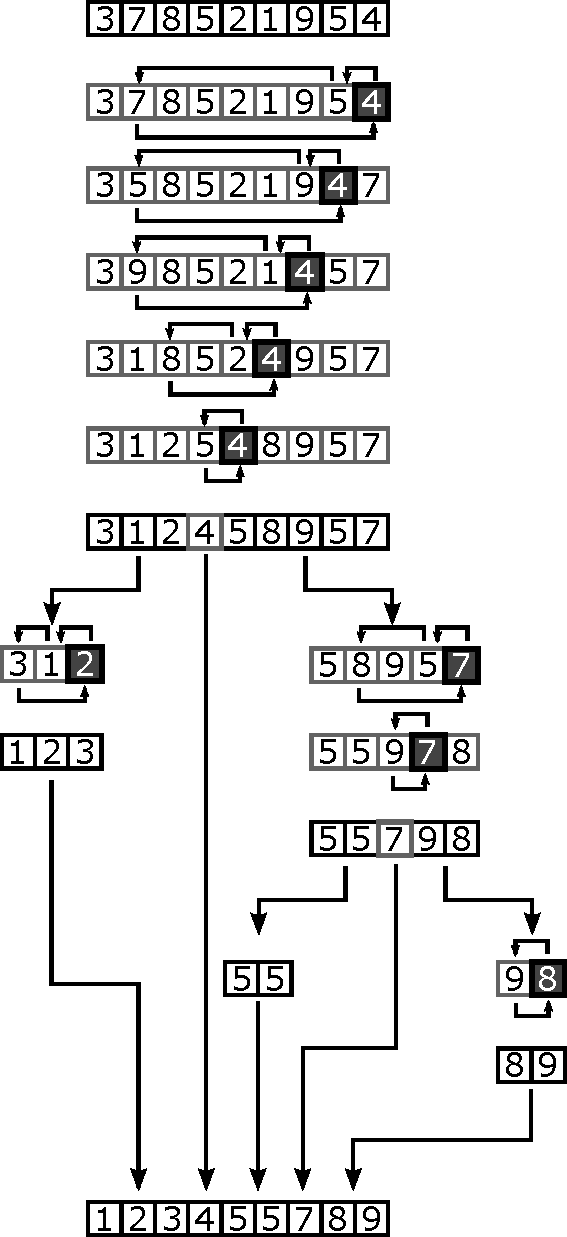
\includegraphics[height=3.0in]{wiki-quicksort-diagram}
\end{center}
\begin{flushright}
{\tiny Image courtesy of Wikipedia.}
\end{flushright}
\end{frame}

{\scriptsize
\begin{frame}[fragile]
\begin{lstlisting}
liftM           :: (Monad m) => (a -> b) -> m a -> m b
liftM f t       = (\y -> return (f y)) >>> t

q               :: (Ord a) => [a]->[a]
q []            = []
q (x:xs)        = q [y|y<-xs,y<x] ++ [x] ++ q [y|y<-xs,y>=x]

main = print >>> (liftM q) getArgs
\end{lstlisting}
\begin{verbatim}

> runghc quicksort.hs f g e d c a b
["a","b","c","d","e","f","g"]
\end{verbatim}
\end{frame}
}

\begin{frame}
\setbeamercovered{dynamic}
    \frametitle{}
    \begin{itemize}
        \item The preceeding page consisted of three lines of executable Haskell
            code. \pause
        \item For the rest of this talk, we will try to understand it,
            from a mathematical point of view. \pause
        \item We must review some category theory first\ldots
    \end{itemize}
\end{frame}

\begin{frame}
\setbeamercovered{dynamic}
    \frametitle{Some Category Theory}
    A \hili{category} \C{} consists of \pause
    \begin{itemize}
        \item a class $\mathrm{obj}(\C)$ of objects \pause
        \item for all objects $A,B,C,\ldots\in \C$ \pause
        \item a set $\Hom_\C(A,B)$ of morphisms \pause
        \item an identity morphism $\mathrm{id}_A \in \Hom_\C(A,A)$ \pause
        \item a composition function \[\Hom_\C(A,B)\times \Hom_\C(B,C)
            \rightarrow \Hom_\C(A,C)\] denoted by $g\circ f$ or $f;g$
            for \[A \xrightarrow{f} B \xrightarrow{g} C\]
    \end{itemize}
\end{frame}

\begin{frame}
\setbeamercovered{dynamic}
    \frametitle{Some Category Theory}
    \begin{itemize}
        \item such that for \[A \xrightarrow{f} B \xrightarrow{g} C
            \xrightarrow{h} D\] we have \[f;(g;h) = (f;g);h\] \pause
        \item and for $f : A \rightarrow B$ we have \[f;id_B = f = id_A;f\]
    \end{itemize}
\end{frame}

\begin{frame}
\setbeamercovered{dynamic}
    \frametitle{Some Category Theory}
    \begin{itemize}
        \item The fundamental example is the category
            of sets, denoted \SET{}
        \begin{itemize}
            \item objects are sets
            \item morphisms are set theoretic functions
            \item composition is composition of set functions, etc
        \end{itemize} \pause
        \item We are interested in the category of Haskell data types
            \typ{}\pause
        \item We will model \typ{} by \SET{}, i.e.~for this talk we
            define \[\typ{} := \SET{}\]
    \end{itemize}
\end{frame}

\begin{frame}
\setbeamercovered{dynamic}
    \frametitle{The Category of Data Types}
    \begin{itemize}
        \item Let us consider \typ \pause
        \item An object is to be a data type\pause
        \item A morphism between data types has as input a data type
            and produces as output a data type\ldots\pause
        \item Thus an algorithm written in Haskell is \hili{defined}
            to be a morphism $f: A \rightarrow B$ in \typ, \pause
        \item and $A \rightarrow B$ is its type signature \pause
        \item There are further requirements to be an algorithm which
            we will ignore for this talk\ldots\pause
        \item Absent a more precise definition, \textit{we know an
            algorithm when we see one.}
    \end{itemize}
\end{frame}

\begin{frame}
\setbeamercovered{dynamic}
    \frametitle{The Category of Data Types}
    \begin{itemize}
        \item Examples of data types:\pause
        \item $\Z$, the integers\pause
        \item $L(\Z)$ := the set of lists of integers\pause
        \item $L(A) $ := the set of lists of type $A$ for $A\in
            \typ$\pause
\begin{align*}
            L(A) & := \bigcup_{n \ge 0} A^n \\
            & = \{(a_1,\dots,a_m) : m < \infty, a_i \in A,\, \forall
            i=1,\dots m\}.
\end{align*}
        \item Strings := Lists of characters\pause
        \item Binary trees with leaves of type $A\in \typ$
    \end{itemize}
\end{frame}

\begin{frame}
\setbeamercovered{dynamic}
    \frametitle{The Category of Data Types}
    \begin{itemize}
        \item We see that $L$ assigns to a data type $A$ a new data
            type, the set of lists on $A$,\pause
        \item thus is some sort of map from \typ{} to \typ{}\pause
        \item We may say that ``List'' is a parametrized data type
    \end{itemize}
\end{frame}

\begin{frame}
\setbeamercovered{dynamic}
    \frametitle{Some Category Theory}
    \begin{definition}
        A functor $F : \C \rightarrow \C'$ from a category \C{} to a
        category \C' is a rule which

        -- given $A\in \C$ produces $F(A) \in \C'$ and

        -- given $f: A \rightarrow B$ in \C, produces $F(f):F(A)
        \rightarrow F(B)$ in \C'

        -- and satisfies various axioms, for instance $F(f;g) = F(f);F(g)$
    \end{definition}
\end{frame}

\begin{frame}
\setbeamercovered{dynamic}
    \frametitle{Some Category Theory}
    \begin{definition}
        Given functors $F : \C \rightarrow \C'$ and $G: \C'\rightarrow
        \C''$ we may compose them to obtain $$F;G : \C \rightarrow
        \C''.$$

        Thus we have the notion of $\End(\C)$, which is the
        category of all endofunctors of \C{}:

        -- the objects are functors $F : \C \rightarrow \C$ (known as
        endofunctors)

        -- the morphisms are natural transformations of functors
    \end{definition}
\end{frame}

\begin{frame}
\setbeamercovered{dynamic}
    \frametitle{Some Category Theory}
    \begin{definition}
        A monad over \C{} is a monoid in $\End(\C)$. By this we mean a
        functor $T \in \End(\C)$ together with natural transformations
        $\mu : T\times T \rightarrow T$ and $\mu : \idc \rightarrow T$
        which satisfy the associativity and unit axioms of a monoid
        {\scriptsize
\begin{equation*}
\xymatrix{
T\times T \times T \ar[d]_{\id_T \times \mu} \ar[r]^-{\mu\times \id_T} & T\times T \ar[d]^{\mu}
 & T\times \idc \ar[r]^-{\id_T\times \eta} \ar@{=}[dr] & T\times T \ar[d]^-{\mu} & \idc \times T \ar[l]_-{\eta \times \id_T}\ar@{=}[ld] \\
T\times T \ar[r]_-{\mu} & T
 & & T }
\end{equation*} }
(here ``$\times$'' indicates the composition of functors, which is the
product structure in $\End(\C)$.)
    \end{definition}
\end{frame}

\begin{frame}
\setbeamercovered{dynamic}
    \frametitle{Some Category Theory}
        \begin{definition} A Kleisli triple over \C{} is a triple
            \[(T,\eta,(\cdot)^*)\] where

        (1) $T : |\C| \rightarrow |\C|$ is an assignment on objects

        (2) $\eta_A : A \rightarrow TA$ is a morphism in \C{}

        (3) $f^* : TA \rightarrow TB$ for given $f : A \rightarrow TB$

        s.t.~the following hold:

        (a) $\eta_A^* = \id_{TA}$

        (b) $\eta_A;f^* = f$ for $f : A\rightarrow TB$

        (c) $f^*;g^* = (f;g^*)^*$ for $f : A \rightarrow TB$ and $g : B
        \rightarrow TC$
\end{definition}
\end{frame}

\begin{frame}
\setbeamercovered{dynamic}
    \frametitle{Some Category Theory}
\begin{theorem}
The notions of Kleisli triple and monad are equivalent.
\end{theorem}\pause
\begin{proof}
Given a Kleisli triple \((T,\eta,(\cdot)^*)\) the corresponding
monad is $(T,\eta,\mu)$ where we make $T$ into an endofunctor by
defining for $f: A\rightarrow B$ \[Tf := (f;\eta_B)^* \text{ and }
\mu_A := \id_{TA}^*.\] \pause

Conversely, given a monad $(T,\eta,\mu)$ we define a Kleisli triple by
restricting the functor $T$ to objects and for $f: A\rightarrow TB$ we
put \[f^* := (Tf);\mu_B.\] \end{proof}
\end{frame}

\begin{frame}
\setbeamercovered{dynamic}
    \frametitle{The List Monad}
    \begin{itemize}
        \item Let us see that the endofunctor $L \in \End(\typ)$ is
            actually a monad.\pause
        \item $L(A) $ := the set of lists of type $A$ for $A\in \typ$
            \begin{align*}
            L(A) & := \bigcup_{n \ge 0} A^n \\
            & = \{(a_1,\dots,a_m) : m < \infty, a_i \in A,\, \forall
            i=1,\dots m\}.
            \end{align*}
   \end{itemize}
\end{frame}

\begin{frame}
\setbeamercovered{dynamic}
    \frametitle{The List Monad}
    \begin{itemize}
        \item An example will tell us how to define the monadic
            ``multiplication'' and ``identity'' $\mu_A : (L\times
            L)(A) := L(L(A))  \rightarrow L(A)$ and $\eta_A : A
            \rightarrow L(A)$\pause
        \item Take $A := \Z$. \pause
            Then \[ ( (1,2), (3), (4,5) ) \xrightarrow{\mu_\Z}
            (1,2,3,4,5)\] removes a layer of parentheses \pause
            and \[n \xrightarrow{\eta_\Z} (n)\] is the
            list consisting of a single element.
    \end{itemize}
\end{frame}

\begin{frame}[fragile]
\setbeamercovered{dynamic}
    \frametitle{Coding the List Monad}
\begin{lstlisting}
instance Monad List where
    return x = [x]
    f >>> xs  = (concat . fmap f) xs
\end{lstlisting}\pause
    \begin{itemize}
        \item \texttt{return x}  is $\eta_A(x)$\pause
        \item \texttt{xs} is a list, so how to define \verb|f >>> xs|? \pause
        \item given $f: A\rightarrow L(B)$ the Kleisli star gives us
            $f^* : L(A) \rightarrow L(B)$, \pause
        \item \texttt{concat} = $\mu_A$, \pause
        \item \texttt{fmap f} = $L(f)$,
    \end{itemize}
\end{frame}

\begin{frame}[fragile]
\setbeamercovered{dynamic}
    \frametitle{Coding the List Monad}
    \begin{itemize}
        \item thus %\verb|(concat . fmap f)| =
        \[\mathtt{\text{( concat . fmap f )}} = \mu_B \circ L(f) = L(f) ; \mu_B
        =: f^*\] \pause
        % \item \verb|f >>> x| comes from the Kleisli star: \pause
        \item and %\verb|f >>> xs| :=
        \begin{align*}
            \mathtt{\text{f \shove{} xs}} & :=  f^*(xs) \\
            & = \mu_B(L(f)(xs))\\
            & = \mu_B ( (f(y) : y\in xs) ) \\
            & = \mathtt{concat} (f(y) : y \in xs)
        \end{align*}
    \end{itemize}
\end{frame}

\begin{frame}[fragile]
\setbeamercovered{dynamic}
    \frametitle{Coding the List Monad}
    \begin{itemize}
        \item An example:
        \item $f : \Z \rightarrow L(\Z)$ \pause
        \item \verb|f n = [n,n^2]| \pause
        \item \verb|f >>> [1..5] =| \pause
        \item \verb|(concat . fmap f) [1..5] =| \pause
        \item \verb|concat (fmap f [1..5]) =| \pause
        \item \verb|concat [[1,1],[2,4],[3,9],[4,16],[5,25]] =| \pause
        \item \verb|[1,1,2,4,3,9,4,16,5,25]|
    \end{itemize}
\end{frame}

\begin{frame}
\setbeamercovered{dynamic}
    \frametitle{The State Monad}
    \begin{itemize}
        \item We model the current state of the world as a pair of strings
            $\mathtt{(is,os)} \in \SS \times \SS$ where \pause
        \item $\SS$ is the set of all strings \pause
        \item \texttt{is} = characters waiting to be read in the input
            stream\pause
        \item \texttt{os} = characters already written to the output
            stream\pause
        \item We define the state monad as an endofunctor of \typ, \(
            T : \typ \rightarrow \typ\) to be \[ T(A) := \HSS{A} \]\pause
        \item One can show that it forms a monad
    \end{itemize}
\end{frame}

\begin{frame}[fragile]
\setbeamercovered{dynamic}
    \frametitle{The State Monad}
    \begin{itemize}
        \item Thus a $f\in T(A)$ assigns to every possible initial
            state of the world $\mathtt{(i,o)}$ a final state
            $(\mathtt{i',o'},\alpha)$\pause
        \item We view $f$ as the action of a single step of an
            algorithm\pause
        \item In case we are reading input, we think of $\alpha$ as
            the value read off of the initial input stream, resulting
            in the final input stream and output stream \pause
        \item In case of printing output, $\alpha$ would be an empty
            value\pause
        \item Example of reading input

            \texttt{i = "def", o = "cba"}

            \texttt{i' = "ef", o' = "cba",} $\alpha$ \texttt{= "d"} \pause
        \item As described earlier, it is in this way that we pass
            around the state of the world as a variable, in a
            referentially transparent manner.
    \end{itemize}
\end{frame}

\begin{frame}[fragile]
\setbeamercovered{dynamic}
    \frametitle{Coding the State Monad}
    Given $f : A\rightarrow T(B)$ and $t\in T(A)$ we define
    \verb|f >>> t| $\in T(B)$ to be\pause \[
    x \mapsto f( \text{return-value}(t(x)) )( \text{new-state}(t(x)) )
    \] \pause where we think of
    \begin{align*}
    T(B) & = \Hom( S, S\times B)\\
    & = \Hom(\text{initial-state}, \text{new-state}\times \text{return-value})
    \end{align*} and $S := \SS\times \SS.$
\end{frame}

\begin{frame}[fragile]
\setbeamercovered{dynamic}
    \frametitle{Back to our three line program}
    %// move this to after the treatment of state monad
    Let us compare the two definitions of Quicksort:
    {\scriptsize
\begin{lstlisting}
q []            = []
q (x:xs)        = q [y|y<-xs,y<x] ++ [x] ++ q [y|y<-xs,y>=x]
\end{lstlisting}

\begin{verbatim}
function Quicksort( Array )
...
return Concatenate( Quicksort( LessThanPivotArray ),
                    Pivot,
                    Quicksort( GreaterThanPivotArray ) )
\end{verbatim}
}
\end{frame}

\begin{frame}[fragile]
\setbeamercovered{dynamic}
    \frametitle{Back to our three line program}
    Let us now consider the function liftM
    {\scriptsize
\begin{lstlisting}
liftM           :: (Monad m) => (a -> b) -> m a -> m b
liftM f xs      = (\y -> return (f y)) >>> xs

... liftM q ...
\end{lstlisting}
}
    \begin{itemize}
        \item Recall from before that we have \verb|f >>> xs| :=
            $\mu_A(L(f)(xs)) = \mu_A ( (f(y) : y\in xs) ) =
            \mathtt{concat} (f(y) : y \in xs)$ \pause
        \item Now, $q : L(A) \rightarrow L(A)$ so that \verb|liftM q|
            is the function \verb|g(xs) = (\y -> return (q y)) >>> xs|
            where \texttt{xs} is a list \pause
        \item \textit{In other words, it is the function which takes a
            list of lists and sorts each of the sublists therein,
            returning the result in list which is the result of
            concatenating all of those sorted sublists!}
    \end{itemize}
    % therefore it needs to be passed a list of lists of strings of
    % the form [ [s1,s2,s3] ] with the s_i strings; thus the action is
    % to sort the inner list and strip an outer layer of parens.
\end{frame}

\begin{frame}[fragile]
\setbeamercovered{dynamic}
    \frametitle{Back to our three line program}
\begin{lstlisting}
getArgs      :: State [String]
print        :: a -> State ()

main = print >>> (liftM q) getArgs
\end{lstlisting}
    \begin{itemize}
        \item We know that \verb|getArgs| is of type \verb|State [String]| \pause
        \item thus it is an assigment which takes the initial
            input/output state and gives us the final input/output
            state as well as a list of strings read off of the input
            \pause
        \item After what we have seen on \verb|liftM q|, we know that
            it simply sorts the list of strings (and strips off a layer
            of parentheses) \pause
        \item Finally, given the initial input/output state, print
            appends the resulting sorted list to the output and
            returns an empty value
    \end{itemize}
\end{frame}

\begin{frame}[fragile]
This is our program, in its entirety.
{\scriptsize
\begin{lstlisting}
import System.Environment

(>>>)           :: (Monad m) => (a -> m b) -> m a -> m b
f >>> x         = x >>= f

liftM           :: (Monad m) => (a -> b) -> m a -> m b
liftM f t       = (\y -> return (f y)) >>> t

q               :: (Ord a) => [a]->[a]
q []            = []
q (x:xs)        = q [y|y<-xs,y<x] ++ [x] ++ q [y|y<-xs,y>=x]

main = print >>> (liftM q) getArgs
\end{lstlisting}
\begin{verbatim}

> runghc quicksort.hs f g e d c a b
["a","b","c","d","e","f","g"]
\end{verbatim} }
\end{frame}

\begin{frame}
\setbeamercovered{dynamic}
\begin{center}
    {\Huge \textcolor{title}{Thank you.}}
\end{center}
\end{frame}

\begin{frame}[fragile]
\begin{verbatim}
-- the true type signatures
getArgs      :: IO [String]
print        :: (Show a) => a -> IO ()
\end{verbatim}
\end{frame}

\end{document}
